\section{Statistical Analysis}

\subsection{Definition of test statistic}
\label{sec:test-statistic}

To make a measurement, the discrepancy between the histograms from re-weighted MC events and observed data events has to be measured by an appropriate test statistic.
This measurement uses a modified $\chi^2$ test statistic defined as
\begin{equation}
\chi^2_{\mathrm{mod}} = \sum_{i \in \mathrm{bins}}^{}\frac{(N^{\mathrm{exp}}_i - N^{\mathrm{obs}}_i)^2}{N^{\mathrm{exp}}_i + (\sigma^{\mathrm{exp}}_i)^2} + \sum_{j \in \mathrm{syst}}^{}\frac{(s_j - \hat{s_j})^2}{\sigma^2_{s_j}},
\label{eq:mod-chi2}
\end{equation}

\noindent where the expectation within a bin is calculated as the sum of the MC event weights $N^{\mathrm{exp}}_i = \sum_{i}^{\mathrm{evts}} w_i$. The error term due to Poisson fluctuations of the data is calculated with the MC expectation, $N^{\mathrm{exp}}_i$. The statistical uncertainty due to finite simulation statistics is also included as $(\sigma^{\mathrm{exp}}_i)^2 = \sum_{i}^{\mathrm{evts}} w_i^2$.
The second term in equation~\ref{eq:mod-chi2} is included as a penalty term to account for prior knowledge of some systematic parameters.


\subsection{Muon KDEs}
\label{section:muon_kde}

After all the filtering steps described in section~\ref{sec:data-processing}, the muon contamination of the data sample is reduced to $\sim 2\%$ of the sample.
This reduces the statistics of muon simulation so much, that the resulting histograms become very sparse as shown in figure~\ref{fig:muon-template-no-kde}.
Such sparse histograms, in which single MC events have to serve as a stand-in for several real data events, are a poor template for what can be expected in data.
To produce a more realistic expectation of the bin counts, the muon histograms are smeared using KDEs as shown in figure \ref{fig:muon-template-with-kde}.
Since the KDE operates on events on the entire zenith and energy range, including events that fall outside the analysis binning, some events bleed into the highest $\cos(\theta_z)$ bin from further above the horizon.
The KDE kernel is mirrored at $\cos(\theta_z) = -1$ to avoid spurious disappearance of events at the edge.

\begin{figure}[H] 
    \centering
    \begin{subfigure}{0.8\textwidth}
        \centering
        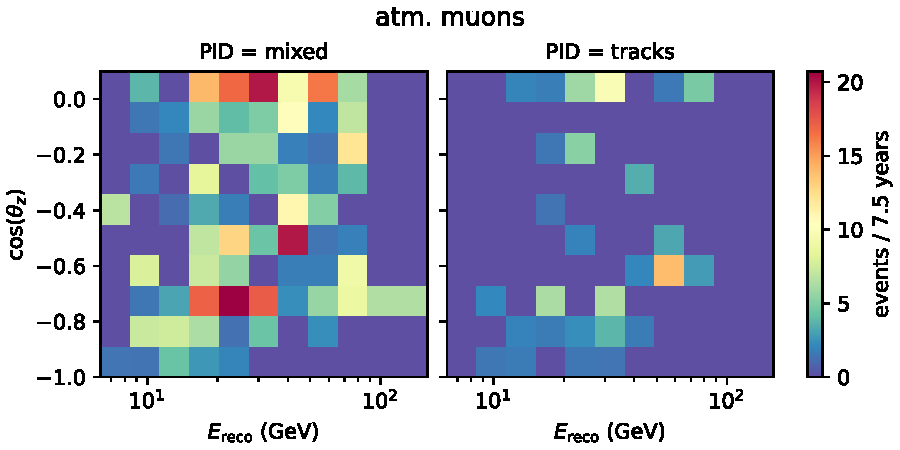
\includegraphics[width=\textwidth,trim={0 0 0 0.6cm},clip]{figures/measurement/systematics/muons/muon_hist_no_kde.pdf}
        \caption{Without KDE smoothing}
        \label{fig:muon-template-no-kde}
    \end{subfigure}
    \begin{subfigure}{0.8\textwidth}
        \centering
        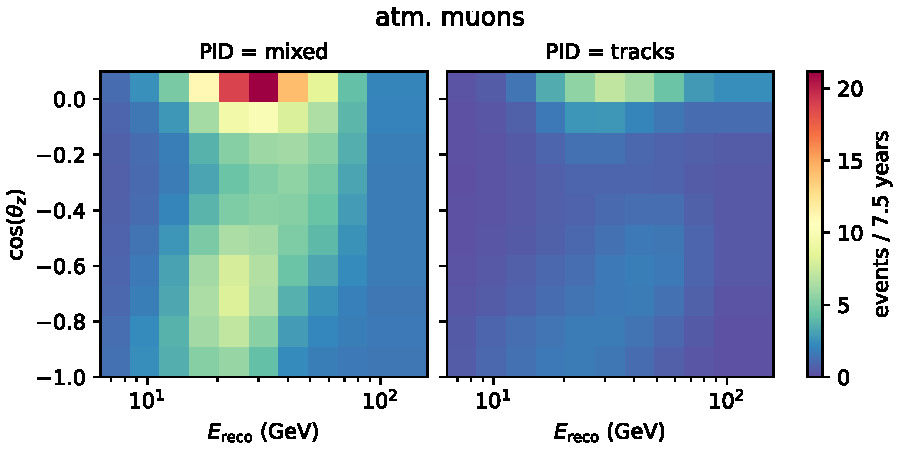
\includegraphics[width=\textwidth,trim={0 0 0 0.6cm},clip]{figures/measurement/systematics/muons/plot_maps_muon.pdf}
        \caption{With KDE smoothing}
        \label{fig:muon-template-with-kde}
    \end{subfigure}
    
    \caption{Muon template before (top) and after (bottom) the application of KDE smoothing. The shown values are the average of 20 KDE evaluations on different bootstrap samples.}
    \label{fig:muon-kde-smoothing}
\end{figure}

\subsubsection{KDE error estimates}
To estimate the error on the KDE output, 20 bootstrap samples are drawn separately in each PID channel and the KDE is re-evaluated for each trial.
The expectation value and standard deviation of the expectation in each bin of the histogram is the mean and standard deviation of these samples, respectively.
The samples are always produced with the same initial random seed to ensure that the expectations and errors are reproducible.